\documentclass[a4paper]{article}
\usepackage[utf8]{inputenc}
\usepackage[nodayofweek]{datetime}

% Set size of text area with total parameter
\usepackage[a4paper, total={185mm, 255mm}]{geometry}

\usepackage{tikz}
\usetikzlibrary{math}
\tikzmath{
	\npi = 3.1415926535897;
	\rtwot = sqrt(2)/2;
	\rthot = sqrt(3)/2;
}
\tikzset{
	asymptote/.style={dashed,semithick}
}

% \asymptote command only good for "vertical asymptote axis"
\newcommand{\verticalAsymptote}[1]{\draw [asymptote] (#1,-4.2) -- (#1,4.2);}

\usepackage{pgfplots}
\pgfplotsset{
	compat=1.18,
	normal trig axis/.style={
		grid=both,
		samples=1000,
		no marks,
		xmax=6.48,
		xmin=-6.48,
		xlabel=$x$,
		ylabel=$y$,
		xtick={-2*\npi,-1.5*\npi,...,2*\npi},
		xticklabels={%
			$-2\pi$,
			$-\frac{3\pi}{2}$,
			$-\pi$,
			$-\frac{\pi}{2}$,
			0,
			$\frac{\pi}{2}$,
			$\pi$,
			$\frac{3\pi}{2}$,
			$2\pi$},
		axis lines=middle
	},
	sin cos axis/.style={
		normal trig axis,
		% Meant to be used in minipage, so full width
		width=\textwidth,
		height=0.8\textwidth,
		ymax=1.2,
		ymin=-1.2,
		ytick={%
			-1,
			-0.5,
			0,
			0.5,
			1},
		yticklabels={%
			-1,
			$-\frac{1}{2}$,
			0,
			$\frac{1}{2}$,
			1}
	},
	vertical asymptote axis/.style={
		normal trig axis,
		ymax=4.2,
		ymin=-4.2,
		ytick={-4,-3,...,4},
		restrict y to domain=-4.5:4.5
	},
	trig plot/.style={
		domain=-2*\npi:2*\npi,
		thick
	}
}

\newcommand{\sectitle}[1]{%
	\vspace*{0.8em}
	\begin{center}
		\Large
		\textsl{\underline{#1}}
		\normalsize
	\end{center}
	\vspace*{0.5em}}

\begin{document}

\begin{center}
	\Huge\textbf{Trig Crib Sheet}\normalsize
\end{center}

\sectitle{Definitions}

\begin{figure}[h]
\begin{minipage}{0.65\linewidth}
\centering
\resizebox{0.8\linewidth}{!}{%
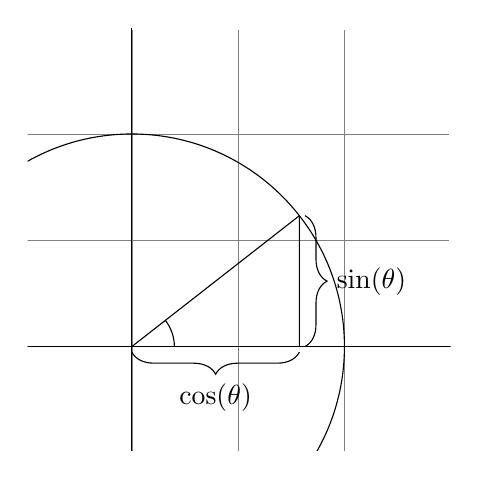
\begin{tikzpicture}[scale=2.7]
	\clip (1.5,1.5) rectangle (-0.49,-0.49);

	\coordinate (O) at (0,0);
	\coordinate (P) at (38:1);
	\coordinate (I) at (P |- O);

	\draw [step=0.5, gray, ultra thin] (1.49,1.49) grid (-1.49,-1.49);

	\draw (-1.5,0) -- (1.5,0) (0,1.5) -- (0,-1.5);
	\draw (0,0) circle[radius=1];

	\draw (0,0) -- (P);
	\draw (P) -- (I);

	\draw (0.2,0) arc[start angle=0, end angle=38, radius=0.2];
	%\draw (0.1,0) node [anchor=south west] {$\theta$};

	\draw [decorate, decoration={brace, amplitude=8pt, raise=2pt}] (P) -- node [right, xshift=10pt] {$\sin(\theta)$} (I);
	\draw [decorate, decoration={brace, amplitude=8pt, mirror, raise=2pt}] (O) -- node [below, yshift=-10pt] {$\cos(\theta)$} (I);
\end{tikzpicture}
}\end{minipage}\hspace{3ex}
\begin{minipage}{0.25\linewidth}
	\large
	$$\tan\theta = \frac{\sin\theta}{\cos\theta}$$
	\vspace{1em}
	$$\sec\theta = \frac{1}{\cos\theta}$$
	\vspace{1em}
	$$\csc\theta = \frac{1}{\sin\theta}$$
	\vspace{1em}
	$$\cot\theta = \frac{1}{\tan\theta} = \frac{\cos\theta}{\sin\theta}$$
\end{minipage}
\end{figure}

\sectitle{Graphs}

\begin{figure}[h]
\centering
\begin{minipage}{0.5\linewidth}
	\begin{tikzpicture}
		\begin{axis}[sin cos axis]
			\addplot [trig plot] {sin(deg(x))};
			\coordinate (title) at (axis cs:0,1.2) {};
		\end{axis}

		\node at (title) [above] {$y = \sin(x)$};
	\end{tikzpicture}
\end{minipage}\hfill
\begin{minipage}{0.5\linewidth}
	\begin{tikzpicture}
		\begin{axis}[vertical asymptote axis]
			\addplot [trig plot] {1/sin(deg(x))};

			\verticalAsymptote{-6.2832}
			\verticalAsymptote{-3.1416}
			\verticalAsymptote{0}
			\verticalAsymptote{3.1416}
			\verticalAsymptote{6.2832}

			\coordinate (title) at (axis cs:0,4.2) {};
		\end{axis}

		\node at (title) [above] {$y = \csc(x)$};
	\end{tikzpicture}
\end{minipage}
\end{figure}

\begin{figure}[h]
\centering
\begin{minipage}{0.5\linewidth}
	\begin{tikzpicture}
		\begin{axis}[sin cos axis]
			\addplot [trig plot] {cos(deg(x))};
			\coordinate (title) at (axis cs:0,1.2) {};
		\end{axis}

		\node at (title) [above] {$y = \cos(x)$};
	\end{tikzpicture}
\end{minipage}\hfill
\begin{minipage}{0.5\linewidth}
	\begin{tikzpicture}
		\begin{axis}[vertical asymptote axis]
			\addplot [trig plot] {1/cos(deg(x))};

			\verticalAsymptote{-4.7124}
			\verticalAsymptote{-1.5708}
			\verticalAsymptote{1.5708}
			\verticalAsymptote{4.7124}

			\coordinate (title) at (axis cs:0,4.2) {};
		\end{axis}

		\node at (title) [above] {$y = \sec(x)$};
	\end{tikzpicture}
\end{minipage}
\end{figure}

\begin{figure}[h]
\centering
\begin{minipage}{0.5\linewidth}
	\begin{tikzpicture}
		\begin{axis}[vertical asymptote axis]
			\addplot [trig plot] {tan(deg(x))};

			\verticalAsymptote{-4.7124}
			\verticalAsymptote{-1.5708}
			\verticalAsymptote{1.5708}
			\verticalAsymptote{4.7124}

			\coordinate (title) at (axis cs:0,4.2) {};
		\end{axis}

		\node at (title) [above] {$y = \tan(x)$};
	\end{tikzpicture}
\end{minipage}\hfill
\begin{minipage}{0.5\linewidth}
	\begin{tikzpicture}
		\begin{axis}[vertical asymptote axis]
			\addplot [trig plot] {1/tan(deg(x))};

			\verticalAsymptote{-6.2832}
			\verticalAsymptote{-3.1416}
			\verticalAsymptote{0}
			\verticalAsymptote{3.1416}
			\verticalAsymptote{6.2832}

			\coordinate (title) at (axis cs:0,4.2) {};
		\end{axis}

		\node at (title) [above] {$y = \cot(x)$};
	\end{tikzpicture}
\end{minipage}
\end{figure}

\end{document}
